



\section{Two level parallelism}

Our current implementation assumes that we are computing on a cluster of CPUs,
with one GPU attached to each CPU. The CPU maintains control of execution and
launches kernels on the GPU that execute in parallel. Under the OpenCL standard
\cite{OpenCL2009}, a tiered memory hierarchy is available on the GPU with
\textit{global device memory} as the primary and most abundant memory space.
The memory space for GPU kernels is separate from the memory available to a
CPU, so data must be explicitly copied to/from global device memory on the GPU. 

\begin{itemize} 
\item How to copy to/from GPU
\item Where are the synchronization points (lockstep and overlapping)
\end{itemize}

\authnote{The basic primitives necessary to parallelize our problems: SpMV, AXPY and }


%\subsection{Overlapping Computation and Communication} 
%Need to describe our approach to launch 
%
%In simplest form (\& indicates an overlapped execution; overlapping is possible by non-blocking launches to the GPU before comm is started): 
%\begin{itemize} 
%\item $ U_{Q \backslash B}' = A_{Q \backslash B} U_{Q \backslash B}$ \& MPI\_alltoallv
%\item $ U_{B}' = A_{B} U_{B}$ 
%\end{itemize} 
%This form benefits because stencils are operated on in their entirety. For the GPU this is important because we maintain SIMD nature. 
%
%A more complex form which might overlap more comm and comp depending on the size of B (i.e., might be beneficial for large stencil sizes): 
%\begin{itemize} 
%\item $ U_{Q \backslash B}' = A_{Q \backslash B} U_{Q \backslash B}$ \& MPI\_alltoallv
%\item \& $ U_{B}' = A_{B \backslash R} U_{B \backslash R}$  (partial sparse vector product)
%\item $ U_{B}' += A_{R} U_{R}$ 
%\end{itemize} 
%
%Note that there is no non-blocking version of MPI\_alltoallv within the MPI standard, so the above two algorithms will not be overlapped when computing on the CPU. To overlap on the CPU, \cite{Kandalla2011} refers to the non-blocking collective as MPI\_ialltoallv. With a collective like this, we could enforce a pattern like: 
%\begin{itemize} 
%\item MPI\_alltoallv
%\item \& $ U_{Q \backslash B}' = A_{Q \backslash B} U_{Q \backslash B}$ 
%\item \& $ U_{B}' = A_{B \backslash R} U_{B \backslash R}$  (partial sparse vector product)
%\item MPI\_wait
%\item $ U_{B}' += A_{R} U_{R}$ 
%\end{itemize} 

%K. Kandalla, H. Subramoni, K. Tomko, D. Pekurovsky, S. Sur and D.K. Panda, "High-performance and scalable non-blocking all-to-all with collective offload on InfiniBand clusters: a study with parallel 3D FFT", Computer Science - Research and Development, vol. 26(3-4):237-246, 2011.
%T. Hoefler, A. Lumsdaine and W. Rehm, "Implementation and Performance Analysis of Non-Blocking Collective Operations for MPI", International Conference for High Performance Computing, Networking, Storage and Analysis (SC07), Reno, USA, 2007.




%\subsubsection{Boundary Conditions} 
%Boundary conditions are handled on the GPU in the following way: 

dirichlet: kernel copies dirichlet values into place \authnote{Need to dust off code}



\subsection{Fragments (integrate above)}


%The term \textit{General Purpose Computing on GPUs} (GPGPU) refers to the application of a Graphics Processing Unit (GPU) 
%to problems other than typical rendering tasks (i.e., vertex transformation, rasterization, etc). Driven by the gaming industry's 
%insatiable desire for more realistic graphics, GPU performance in the last decade years has grown tremendously compared to CPUs.

%Based on \cite{Jansen:2007, CudaGuide:2008, GTX280:2008, Core2Extreme:2008, FermiPrice:2009}, we see in Figure~
%\ref{fig:gpuevolution} the widening gap between compute capabilities on 
%the GPU and CPU. The latest GPUs are capable of approximately ten times the number of 
%floating point operations per second compared to the latest generation CPU. Naturally, this peak 
%performance comes with limitations: historically GPUs have always lagged behind the CPU in terms 
%of flexibility and programmability.

While the nomenclature used in this paper is typically associated with CUDA programming, the names \textit{thread} and \textit{warp} are used to clearly illustrate kernel execution in context of the NVidia specific hardware used in tests. OpenCL assumes a lowest common denominator of hardware capabilities to provide functional portability. However, intimate knowledge of hardware allows for better understanding of performance and optimization on a target architecture. For example, OpenCL assumes all target architectures are capable at some level of SIMD (Single Instruction Multiple Data) execution, but CUDA architectures allow for Single Instruction Multiple Thread (SIMT). SIMT is similar to traditional SIMD, but while SIMD immediately serializes on divergent operations, SIMT allows for a limited amount of divergence without serialization. 

At the hardware level, a \textit{thread} executes instructions on the GPU. On Fermi level GPUs, groups of 32 threads are referred to as \textit{warps}. A warp is the unit of threads executed concurrently on a single \textit{multi-processor}. 
In OpenCL (i.e., software), a collection of hardware threads performing the same instructions are referred to as a \textit{work-group} of \textit{work-items}. Work-groups execute as a collection of warps constrained to the same multiprocessor. Multiple work-groups of matching dimension are grouped into an \textit{NDRange}. The \textit{kernel} provides a master set of instructions
for all threads in an NDRange \cite{OpenCL2009}. 

%\authnote{Just rewrote this stuff directly in opencl terms}
%In software, a collection of threads is referred to as \textit{block}. In hardware, blocks exist as a collection of warps with the constraint that the entire collection executes on the same multiprocessor. Again in software, multiple 
%blocks of matching dimension are grouped into a \textit{grid}. The \textit{kernel} provides a master set of instructions
%for all threads in a grid, although each thread executes the instructions on different memory \cite{CudaGuide:2011}. 

%While the nomenclature used in this paper is typically associated with CUDA programming, the names \textit{thread} and \textit{warp} are used to clearly illustrate kernel execution in context of the NVidia specific hardware. OpenCL has one-to-one mappings for CUDA terminology at the software level, so the two can be used interchangeably. For example, OpenCL labels threads as \textit{work-items}. Blocks are \textit{work-groups}, and a grid is an \textit{NDRange} with an associated \textit{kernel} for an instruction set . 

NVidia GPUs have a tiered memory hierarchy related to the grouping of threads described above. 
In multiprocessors, each computing core executes a thread with a limited set of registers. The number of registers varies with the generation of hardware, but always come in small quantities (e.g., 32K shared by all threads of a multiprocessor on the Fermi). Accessing registers is free, but keeping data in registers requires an effort to maintain balance between kernel complexity and the number of threads per block. Threads of a single work-group can share information within a multiprocessor through \textit{shared memory}. With only 48 KB 
available per 
multiprocessor \cite{CudaGuide2011}, shared memory is another fast but limited resource on the GPU. OpenCL refers to shared memory as \textit{local memory}. 
Sharing information across multiprocessors is possible in \textit{global device memory}---the largest and slowest memory space on the GPU. To improve seek times into global memory, Fermi level architectures include L1 on each multiprocessor and a shared L2 cache for all multiprocessors.


%\textit{constant} and \textit{texture} memory caches are available for read-only access. 
%To use shared memory, 
%Threads must 
%explicitly copy intermediate computational results or data in and out. 

%Shared memory is divided evenly into 16 \textit{memory 
%banks} or 
%regions of memory that can be accessed simultaneously. Memory and registers can be accessed equally fast as long as no two 
%threads in the 
%same half-warp (i.e., first 16 threads or last 16 threads of the warp) are accessing the same memory bank. If this occurs, the 
%access is 
%considered to be a \textit{bank conflict} and the multiprocessor is forced to serialize memory access, increasing the delay until 
%the warp can 
%proceed with execution \cite{CudaGuide:2008}. 

%\begin{figure}[t] %  figure placement: here, top, bottom, or page
%   \centering
%   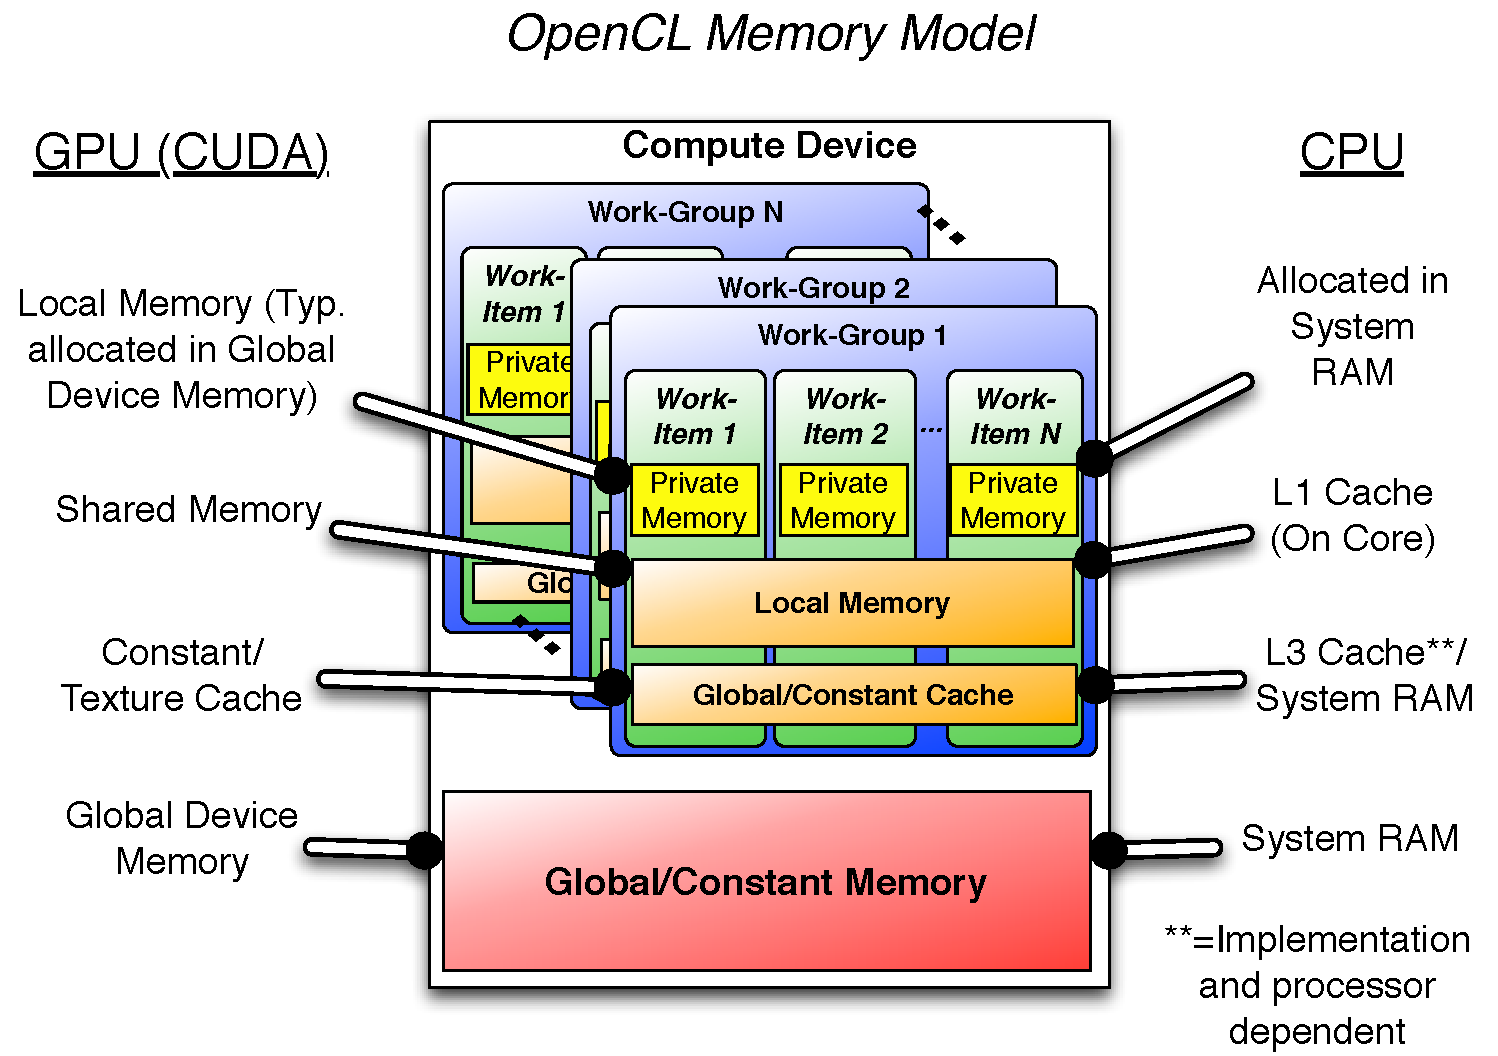
\includegraphics[width=4.5in]{../figures/paper1/figures/opencl_memory_model.pdf} 
%   \caption{Comparison of GPU and CPU implementations underlying the OpenCL memory model for a single compute device.}
%   \label{fig:opencl_memory}
%\end{figure}
%


% and the place to which all data and kernels from the 
%CPU are copied for 
%execution. Note 
%that multiprocessors maintain read-only \textit{caches} for \textit{constants} and \textit{textures}---constants are values that 
%never change during kernel execution, 
%while textures are interpreted as read only arrays and provide a sophisticated cache mechanisms for certain types of non-sequential access. The real memory for constants and textures is part of the global device 
%memory, so reading 
%from texture and constant memory is faster than reads from global memory when no cache misses \cite{CudaGuide:2008}. 
%Also, if a kernel 
%uses too many registers per thread, \textit{local memory} is reserved in the global device memory to temporarily store register 
%contents for 
%later use with an associated penalty in efficiency \cite{CudaGuide:2008}. 

%Under OpenCL, the equivalent to CUDA local memory is called \textit{private memory} and is also reserved read-only per work-item in global device memory. CUDA's shared memory is labeled \textit{local memory} and shared by threads of a work-group. The CUDA texture and constant caches are known as \textit{Global/Constant Cache}, and similar to CUDA, exist outside of developer control. OpenCL refers to \textit{global memory} and \textit{constant memory} when referring to read/write and read-only sections of CUDA's global device memory (respectively). Finally, CUDA textures are equivalent to OpenCL \textit{buffers} (1D arrays) or \textit{images} (2D/3D arrays) \cite{OpenCL:2009}.

%Based on \cite{Behr:2009, OpenCL:2009}, Figure~\ref{fig:opencl_memory} compares the underlying implementation of the OpenCL memory hierarchy on GPUs and CPUs. Notably, on current CPUs most of the memory is reserved in System RAM, whereas the hierarchy naturally fits on the deep memory hierarchy of the GPU.  

\subsection{Implicit Solvers}

Perhaps this section should move up. I think it might be best to discuss GMRES and iterative methods before Distributed Solvers (that way we can say the general solution form is ``matrix form''. but in parallel we need to use distributed algorithms.

The GMRES algorithm follows Algorithm~\ref{alg:gmres_general}. 

The Arnoldi process can be completed using in a variety of ways. Some libraries like CUSP and \cite{Saad2003} prefer the straightforward Givens rotations because they are easily parallelizable. The givens algorithm is provided in Algorithm~\ref{alg:gmres_givens}

Others like [...] prefer to use an alternate algorithm. This algorithm is demonstrated in Algorithm~\ref{alg:gmres_h}.

Parallelizing the algorithm is possible with communication points listed in red (*). 





Alright, starting here.


Itasca

An Alltoall collective shares .... as in Figure~\ref{fig:mpi_alltoall_visual}. A basic Alltoall collective would work in most cases. However, RBF-FD stencils are not required/guaranteed to be symmetric. As a result, we often have non-uniform sharing across partitions, so an Alltoall would require over-padding all send/receive buffers to allow the maximum receive size times the number of processors. 

In order to avoid excessive padding, we choose the Alltoallv collective, which allows processors to share non-uniform number of bytes with one another. Figure~\ref{fig:mpi_alltoallv_visual} illustrates the benefit of Alltoallv in comparison to Alltoall (Figure~\ref{fig:mpi_alltoall_visual}. By allowing variable number of bytes, the total message size is reduced for all processors. The downside to an alltoallv




The data in the Itasca scaling figures considers the case where an MPI\_Alltoallv or MPI\_Isend/MPI\_Irecv is used. By issuing the receives before encoding the send buffers we ensure that no processes wait unnecessarily long for their collectives to start.

When overlapping GPU computation and communication we further reduce the cost of collectives 
Note that the overlapping GPU optimization to reduce the collective times also applies here. We can cut the cost of communication by avoiding the transcribe after the receives have completed. 


\section{On the use of libraries for parallel solvers}

\authnote{$\rightarrow$} 
Implementations of RBF methods are known to be in PETSC \cite{Yokota2010}. The method is simple, and straight-forward to code, but the majority of implementations exist in MATLAB. MATLAB is justified as a platform for computing due to its plethora of solvers, preconditioners, toolkits and support for all things ``matrices" (as it should with a name like ``MATrix LABoratory" (MATLAB). MATLAB is a wonderful platform to develop new features for the RBF methods, but the efficiency of the platform limits its ability to scale to very large problems. For such cases the developers recommend implementations in C or FORTRAN. To aid development in C/FORTRAN, one can take full advantage of the decades worth of research in

Since our focus within this work is to lay the foundation for parallel computing
with RBF-FD, we have made several simplifying assumptions in our code design.
Libraries like PETsc, Hypre, Trilinos and Deal.ii distribute sparse matrix
operations in similar fashion to our approach. When work initially began on this
dissertation, none of these competing libraries contained support for the GPU.
PETsc is currently developing support for the GPU, but we have not had the
chance to consider it yet. 

Our codebase began as a prototype demonstrating the feasibility of RBF-FD
operating on the GPU. Starting from the perspective of RBF-FD as a Lagrangian
method with stationary nodes, the code was developed as $N$ independent dot
products of weights and solution values to approximate derivatives. Weights were
stored linearly in memory, with the solution values read randomly. On the GPU,
stencils were evaluated independently by threads, or shared by a warp of
threads. Operating on stencils in this way implied that GPU kernels were to be
hand written, tuned and optimized. 

Much later, our perspective evolved to see derivative approximation and
time-stepping as sparse matrix operations. This opened new possibilities for
optimization and allowed us to forego hand optimization and fine-tuning of GPU
kernels. With all of the effort put into optimizing sparse operations within
libraries like CUSP \cite{Bell2009}, ViennaCL \cite{Rupp2010} and even the
NVidia provided CUSPARSE \cite{CUSPARSE}, formulating the problem in terms of
sparse matrix operations allows us to quickly prototype on the GPU and leverage
all of the optimizations available within the third party libraries. 

In the most recent version of ViennaCL a set of auto-tuning options were
introduced. We have not investigated these options, but the idea is that they
would only improve the efficiency of our code. 


